\section{Method}
\label{sec:method}

\subsection{Detector}

We use Ultralytics YOLOv8 \citep{jocher2023ultralytics} at two depths,
\texttt{yolov8s} and \texttt{yolov8n}, both with a single-class head. Models are
initialised from COCO-pretrained weights and fine-tuned for $75$ epochs at
$640\times640$, batch $8$, with the Ultralytics default augmentation recipe and
early-stopping patience $20$. The \texttt{s} model is trained with seeds
$0,1,2$; the \texttt{n} model with seed $0$ only, as a single size point. All
runs use the same pinned stack (Ultralytics 8.4.117, PyTorch 2.6.0+cu124) on one
RTX~4070 Laptop GPU with $8$\,GB of memory.

Checkpoint selection is done on validation. For each seed we keep the checkpoint
(last or best) that gives the better validation operating point, then choose the
confidence threshold on validation and apply it unchanged to test. No test
quantity influences any choice. This is the only point in the protocol where
discipline costs something: for some seeds the validation-optimal threshold
transfers badly to test, and we do not fix that after the fact
(Section~\ref{sec:twostage}).

\subsection{Operating points}

For a set of detections, precision $P$, recall $R$ and false positives per image
$\mathrm{FP/img}$ are all functions of a confidence threshold. We define two
operating points on validation and carry both to test:

\begin{itemize}[leftmargin=1.2em,itemsep=2pt]
\item \textbf{Recall-first ($\mathrm{OP}_{97}$).} The largest confidence whose
validation box recall is at least $0.97$. This is the operating point a
demining workflow would plausibly choose: a missed mine is a safety event, a
false alarm is an analyst cost. It is the primary point in all tables.
\item \textbf{High-precision ($\mathrm{OP}_{95}$).} The largest confidence with
validation recall at least $0.95$, used only for the image-level comparison.
\end{itemize}

mAP is computed in the usual way at a low confidence floor ($0.001$) and reported
for comparability with the literature. It plays no role in any selection.

\subsection{Two-stage pipeline}

The second stage is a MobileNetV3-Large classifier \citep{howard2019mobilenetv3}
applied to detector crops. We keep the torchvision
\texttt{mobilenet\_v3\_large} convolutional trunk with ImageNet weights and
replace the classification head with a $128$-unit bottleneck (global average
pool, linear $128$ with ReLU, dropout $0.3$, linear $1$), yielding
$3{,}119{,}535$ parameters in total. Each detection box is expanded by $20\%$ on
each side, cropped, and resized to $224\times224$; the classifier outputs a single
sigmoid score. Training crops are $11{,}550$ positives and $15{,}411$ negatives, the
latter comprising random background, $3{,}730$ detector false positives mined at
confidence $0.05$ from an epoch-20 checkpoint, and $20$ empty-frame samples.
Positives and negatives are sampled $1{:}1$ per epoch; the classifier is
fine-tuned end-to-end for $30$ epochs at learning rate $2\times10^{-5}$ with an
unweighted binary cross-entropy loss. No class weighting is needed here, because
the $1{:}1$ crop sampling already balances the batch; this is the opposite of the
image-level baseline, which is trained on the raw $3{,}887{:}20$ positive-negative
split and therefore requires per-sample weights $[97.7, 0.50]$
(Section~\ref{sec:imagelevel}). The $1{:}1$ ratio and the unfrozen-late-layers
recipe were chosen on validation, and a five-variant ablation is reported in
Section~\ref{sec:ablation}.

We compare three arms, all evaluated on test exactly once with validation-frozen
parameters:

\begin{itemize}[leftmargin=1.2em,itemsep=2pt]
\item \textbf{A (deploy).} YOLO at its validation-chosen
$\mathrm{OP}_{97}$ confidence.
\item \textbf{B (matched recall).} YOLO at the confidence that matches arm C's
\emph{validation} recall. This compares the two-stage arm with a YOLO-only
baseline at the same validation recall and isolates the classifier's contribution
from a trivial threshold change.
\item \textbf{C (two-stage).} YOLO proposals at a fixed low confidence
($0.05$) are routed through the classifier; a proposal is kept if it passes
either a \emph{protection} rule (detector confidence $\ge P$) or the classifier
threshold $\tau$. $P$ is swept over $\{0.4, 0.6, 0.8, \infty\}$ on validation;
for each $P$ we take the largest $\tau$ whose validation recall is within $0.5$
points of stage-1 recall, then choose the pair with the lowest validation
FP/image. Four of the five seeds select $P=0.4$, with
$\tau = 0.27 / 0.23 / 0.22 / 0.13$ for seeds $0/1/2/3$. Seed $4$ selects $P=0.8$
with $\tau = 0.03$, the one place where the rule leaves the $P=0.4$ regime;
Section~\ref{sec:twostage} shows that this choice is what makes arm C regress at
that seed, and we report it rather than overriding it.
\end{itemize}

The protection rule matters. Without it the classifier can veto a
high-confidence detection, and on this corpus that costs recall on the
multi-object \texttt{Jan} source. With $P=0.4$ the pipeline is allowed to
suppress only low-confidence proposals, which is the regime where the
classifier's crop evidence is useful. The rule's weakness is the opposite case:
a high $P$ with a very low $\tau$ leaves almost every proposal protected, so the
classifier is present but inert while still satisfying the recall constraint.

Figure~\ref{fig:pipeline} shows the three arms as data flow. Arms A and B are
scoring rules applied to the same detector run; only arm C adds parameters. The
protection branch is a bypass around the classifier, not a gate in front of it,
which is why a high $P$ can make arm C collapse into arm A without changing any
classifier weight.

\begin{figure*}[t]
\centering
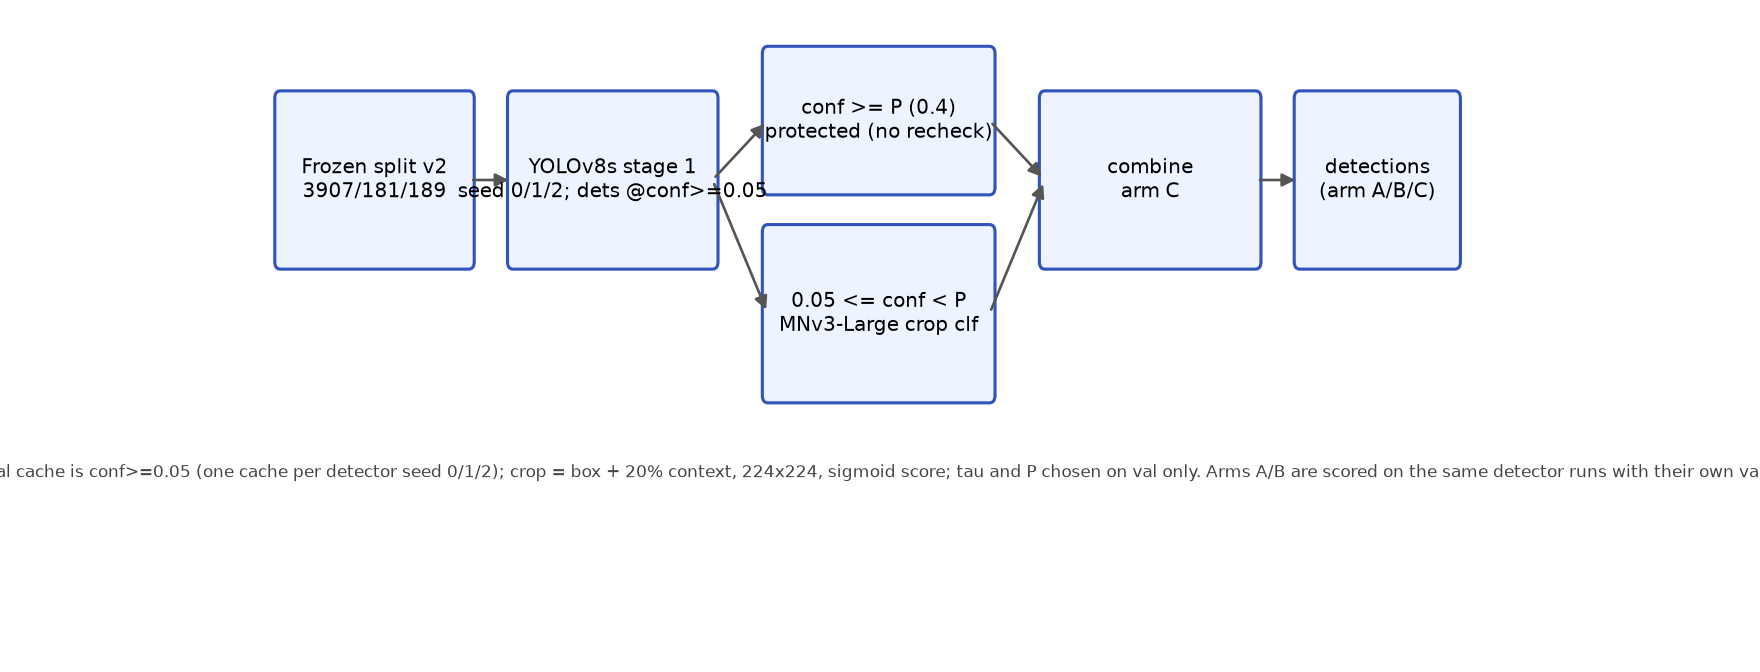
\includegraphics[width=0.88\linewidth]{figs/pipeline.png}
\caption{The two-stage pipeline as data flow. The detector proposes at a low
confidence ($0.05$); a proposal either bypasses the classifier when its detector
confidence is at least the protection threshold $P$, or is scored by the
MobileNetV3-Large crop classifier and compared against $\tau$. Both $P$ and
$\tau$ are chosen on validation. Arms A and B are the same detector run scored by
a single confidence, so the schematic differs between arms only in where the
final comparison happens, not in the features computed.}
\label{fig:pipeline}
\end{figure*}

\subsection{Statistics}

All test comparisons use the same $189$ images, so we resample images, not
detections. For a paired comparison between two arms we draw $5{,}000$ bootstrap
replicates of the image set \citep{efron1993bootstrap} and report the $95\%$
percentile interval of the difference. For single-arm uncertainty we additionally
report a source-cluster bootstrap over the three test sources, and a
leave-one-source-out analysis; with three clusters these intervals are wide by
construction, and we present them as such rather than as precise estimates.
Image-level agreement uses Cohen's $\kappa$ \citep{cohen1960kappa} alongside
balanced accuracy, because the test set has only $5$ negative images and raw
accuracy is dominated by the positive class.

\subsection{Attribution audit}

We compute Grad-CAM \citep{selvaraju2017gradcam} on the neck feature maps feeding
the detection head, targeting the top pre-NMS class score, and on the last
convolutional block of the classifier. Because the top pre-NMS anchor usually
sits on the stride-8 head, the largest stride with a non-zero gradient is used;
this deviates from the common stride-32 choice and is documented with the code.
We report four quantities: the share of CAM energy inside the ground-truth box
(and its enrichment over the box's area share), whether the CAM peak falls inside
the box, the drop in detection score when the box is masked versus when a
matched background region is masked, and a head-to-head comparison of detector
and classifier saliency on the same crops. Every sentence about these numbers is
phrased as evidence about \emph{where the model looked}, never about whether the
prediction is correct.
